\documentclass[10pt,a4paper]{article}

\usepackage[a4paper,left=0.68in,right=0.68in,top=0.62in,bottom=0.60in,headheight=13pt]{geometry}
\usepackage[T1]{fontenc}
\usepackage{lmodern}
\usepackage{microtype}
\usepackage{amsmath,amssymb,mathtools}
\usepackage{booktabs}
\usepackage{enumitem}
\usepackage{xcolor}
\usepackage{tikz}
\usetikzlibrary{arrows.meta,positioning,calc,fit,shapes.geometric}
\usepackage{caption}
\usepackage{fancyhdr}
\usepackage{titlesec}
\usepackage[hidelinks]{hyperref}
\usepackage{multicol}

\pagestyle{fancy}
\fancyhf{}
\lhead{Department of Computer Science and Engineering}
\rhead{DKG-Free Threshold Schnorr Signatures}
\cfoot{\thepage}

\titleformat{\section}{\large\bfseries}{\thesection.}{0.4em}{}
\titleformat{\subsection}{\normalsize\bfseries}{\thesubsection}{0.35em}{}
\setlist[itemize]{leftmargin=1.35em,itemsep=1pt,topsep=1pt}
\setlength{\parindent}{0pt}
\setlength{\parskip}{2pt}
\captionsetup{font=small,labelfont=bf}
\setlength{\abovedisplayskip}{5pt}
\setlength{\belowdisplayskip}{5pt}
\setlength{\abovedisplayshortskip}{2pt}
\setlength{\belowdisplayshortskip}{2pt}

\newcommand{\Zq}{\mathbb{Z}_q}
\newcommand{\G}{\mathbb{G}}
\newcommand{\ip}[2]{\left\langle #1,#2\right\rangle}
\newcommand{\CPK}{C_{\mathsf{PK}}}
\newcommand{\pkpad}{\mathbf{pk}_{\mathrm{pad}}}
\newcommand{\Id}{\mathcal{O}}
\newcommand{\IPA}{\pi_{\mathsf{IPA}}}

\begin{document}

% ============================================================
% TITLE PAGE
% ============================================================
\thispagestyle{empty}

\begin{center}

\vspace*{0.45cm}

{\Large\bfseries
INDIAN INSTITUTE OF INFORMATION TECHNOLOGY\\
DESIGN AND MANUFACTURING KURNOOL
}

\vspace{0.25cm}

{\normalsize
Department of Computer Science and Engineering
}

\vspace{1.25cm}

{\Large\bfseries MID-SEMESTER PROJECT REPORT}

\vspace{0.6cm}

\rule{0.78\textwidth}{0.6pt}

\vspace{0.65cm}

{\LARGE\bfseries
DKG-Free Threshold Schnorr Signatures
}

\vspace{0.35cm}

{\large
\textit{with NUMS-Linked Pedersen Commitments\\
and Inner-Product Arguments}
}

\vspace{0.65cm}

\rule{0.78\textwidth}{0.6pt}

\vspace{0.8cm}

{\normalsize
A report submitted in partial fulfilment of the requirements\\
for the award of the degree of
}

\vspace{0.35cm}

{\Large\bfseries
Bachelor of Technology
}

\vspace{0.15cm}

{\large
Computer Science and Engineering
}

\vfill

{\large\bfseries
Submitted by
}

\vspace{0.35cm}

\renewcommand{\arraystretch}{1.35}

\begin{tabular}{c l}
\textbf{123CS0009} & \textbf{Rineet Pandey}\\
\textbf{123CS0056} & \textbf{Kumar Bhaskar}\\
\textbf{123CS0064} & \textbf{Arnav Sharda}
\end{tabular}

\vspace{1.0cm}

{\large\bfseries
Project Supervisor
}

\vspace{0.3cm}

{\large
Dr. R. KABALEESHWARAN
}

\vfill

\rule{0.55\textwidth}{0.4pt}

\vspace{0.35cm}

{\normalsize
Department of Computer Science and Engineering\\
Indian Institute of Information Technology Design and Manufacturing Kurnool\\
Kurnool, Andhra Pradesh -- 518008
}

\vspace{0.35cm}

{\normalsize
September 2026
}

\end{center}


\newpage

% ============================================================
% 1. INTRODUCTION
% ============================================================
\section{Introduction}

Threshold signatures allow a subset $S$ of participants to jointly authorize
a message provided that $|S|\geq t$. Conventional threshold constructions
typically rely on a shared secret established through a dealer or Distributed
Key Generation (DKG).

This work investigates a \textbf{DKG-free threshold Schnorr construction} in
which participants retain independent secret keys and the threshold condition
is verified using a zero-knowledge proof. The protocol is designed around
independent participant keys, Schnorr signing, silent setup, and a
zero-knowledge threshold proof.

Let $\G$ be a cyclic group of prime order $q$ with generator $G$, and let
$\Zq$ denote its scalar field. The protocol uses domain-separated hash
functions
\[
H_{\mathrm{key}},\quad
H_{\mathrm{non}},\quad
H_{\mathrm{sig}},\quad
H_{\mathrm{link}},
\]
modeled as independent random oracles, with NUMS generators obtained through
domain-separated hash-to-curve procedures.

Each participant $P_i$ generates
\[
sk_i\xleftarrow{\$}\Zq,
\qquad
PK_i=sk_iG,
\]
and publishes a Schnorr proof of possession $\pi_{\mathsf{PoP},i}$. The
registered roster and threshold are bound by
$$C_{PK} = \sum_{i=1}^n H_{key}(pk_i) \pmod q$$
Thus, the protocol obtains a fixed roster and threshold context without
requiring an online common-secret generation phase.

% ============================================================
% 2. LITERATURE REVIEW
% ============================================================
\section{Literature Review}

FROST provides a two-round threshold Schnorr protocol based on distributed
secret shares \cite{FROST}. MuSig2 provides two-round Schnorr multi-signatures
using independently generated keys, but does not directly provide general
$t$-of-$n$ threshold authorization \cite{MuSig2}.

Threshold ECDSA relies on MPC for its non-linear signing operations, while
Threshold BLS uses pairing-based algebra and secret sharing
\cite{GennaroGoldfeder,ThBLS}. The \emph{hinTS} construction is particularly
relevant as a \textbf{silent-setup} threshold signature scheme: participants
can contribute locally generated keys without an online DKG, with succinct
proofs used to establish the well-formedness of the aggregated key
\cite{hinTS}.

Bulletproofs motivate logarithmic inner-product proofs, while KZG provides an
alternative compact polynomial-commitment approach
\cite{Bulletproofs,KZG}.

\begin{table}[h]
\centering
\scriptsize
\renewcommand{\arraystretch}{1.12}
\setlength{\tabcolsep}{3pt}
\begin{tabular}{p{0.20\textwidth}ccccc}
\toprule
\textbf{Property} & \textbf{FROST} & \textbf{ECDSA} &
\textbf{BLS} & \textbf{MuSig2} & \textbf{Proposed}\\
\midrule
Common secret / shares
& Yes & Yes & Yes & No & \textbf{No}\\
DKG / common-secret setup
& Yes & Setup/MPC & Typically yes & No & \textbf{No}\\
Silent setup
& No & Varies & Varies & Yes & \textbf{Yes}\\
Independent keys
& No & Generally no & Generally no & Yes & \textbf{Yes}\\
Dynamic signer selection
& No & Varies & Varies & No & \textbf{Yes}\\
$t$-of-$n$ threshold
& Yes & Yes & Yes & No & \textbf{Yes}\\
Schnorr-based
& Yes & No & No & Yes & \textbf{Yes}\\
Pairings
& No & No & Yes & No & \textbf{No}\\
\bottomrule
\end{tabular}
\caption{Compact architectural comparison of representative constructions.}
\label{tab:comparison}
\end{table}

% ============================================================
% 3. RESEARCH GAPS
% ============================================================
\section{Research Gaps}

Existing schemes provide threshold signing, independent-key Schnorr
aggregation, or silent setup, but these properties are not combined in the
same Schnorr-based construction.

The proposed research addresses the following gap:
\[
\boxed{
\text{Independent Keys}
+\text{ Schnorr Signing}
+\text{ Silent / DKG-free Setup}
+\text{ ZK Threshold Proof}
}
\]

The key relation extracted from the signing transcript is
\[
Q=c^{-1}(sG-R)=\sum_{i\in S}PK_i,
\]
and the zero-knowledge layer must establish that
\[
|S|\geq t
\]
without revealing the signer set. This is achieved using a private binary
signer mask, a NUMS-linked commitment, and a logarithmic inner-product
argument.

% ============================================================
% 4. PROBLEM STATEMENT
% ============================================================
\section{Problem Statement}

The problem addressed in this work is to construct a threshold Schnorr
signature mechanism in which participants can use independently generated
secret keys without requiring an online DKG or a shared secret.

Given $n$ registered participants and a threshold $t$, an active subset
$S\subseteq\{1,\ldots,n\}$ should be able to jointly produce a Schnorr
signature for a message $m$ whenever
\[
|S|\geq t.
\]

The resulting transcript should allow extraction of the aggregate public-key
target
\[
Q=c^{-1}(sG-R)=\sum_{i\in S}PK_i,
\]
while the zero-knowledge proof should demonstrate the threshold condition
without revealing the signer set.

The construction therefore needs to simultaneously address:
\begin{itemize}
\item independent participant keys;
\item two-round Schnorr signing;
\item DKG-free or silent setup;
\item binding of the threshold witness to the registered public keys; and
\item logarithmic-size zero-knowledge proof verification.
\end{itemize}

% ============================================================
% 5. PROPOSED SOLUTION
% ============================================================
\section{Proposed Solution}

\subsection{Two-round Schnorr signing}

Let $S\subseteq\{1,\ldots,n\}$ be the active signing set with $|S|\ge t$.
In Round 1, every signer samples independent one-time nonces
\[
k_{1,i},k_{2,i}\xleftarrow{\$}\Zq,
\qquad
R_{1,i}=k_{1,i}G,\quad R_{2,i}=k_{2,i}G,
\]
and the aggregator computes
\[
R_1=\sum_{i\in S}R_{1,i},\qquad
R_2=\sum_{i\in S}R_{2,i}.
\]

In Round 2,
\[
\beta=H_{\mathrm{non}}(\CPK\|R_1\|R_2\|m),\qquad
R=R_1+\beta R_2,
\]
\[
c=H_{\mathrm{sig}}(\CPK\|R\|m),
\qquad
s_i=k_{1,i}+\beta k_{2,i}+csk_i\pmod q.
\]

For the aggregate
$s=\sum_{i\in S}s_i$,
\begin{align}
sG&=\sum_{i\in S}(k_{1,i}+\beta k_{2,i}+csk_i)G\\
&=R_1+\beta R_2+c\sum_{i\in S}PK_i\\
&=R+c\sum_{i\in S}PK_i.
\end{align}

Hence the target point extracted from the signature transcript is
\[
Q=c^{-1}(sG-R)=\sum_{i\in S}PK_i.
\]

\subsection{Threshold witness encoding}

Let $b\in\{0,1\}^n$ be the signer mask, with $b_i=1$ exactly when
$i\in S$. Define the threshold surplus
\[
v=\sum_{i=1}^{n}b_i-t.
\]
Let $d$ be the binary representation of $v$. For
\[
N=2^{\lceil\log_2(n+m)\rceil},
\]
construct
\[
a_L=b\|d\|0^{N-n-m},\qquad
a_R=a_L-\mathbf1_N.
\]

The mask selects public keys, while the binary surplus encodes the threshold
condition $v\ge0$.

\subsection{NUMS-linked Pedersen commitment}

Choose
$s_L,s_R\xleftarrow{\$}\Zq^N$
and
$\alpha,\rho\xleftarrow{\$}\Zq$.
Form
\[
A=\alpha H_0+\ip{a_L}{G_{\mathrm{nums}}}
+\ip{a_R}{H_{\mathrm{nums}}}.
\]

For the padded public-key vector $\pkpad$,
\[
Q_s=\ip{s_L}{\pkpad},
\]
and the linking challenge is
\[
c_{\mathrm{link}}=
H_{\mathrm{link}}(\mathbf{pk}\|Q\|t\|A\|S\|Q_s).
\]

The NUMS bases are shifted to
\[
G_i'=G_{\mathrm{nums},i}
+c_{\mathrm{link}}\,\mathbf{pk}_{\mathrm{pad},i}.
\]

This step binds the threshold witness to the registered key vector without
abandoning the linear group relation needed by the IPA.

\subsection{Protocol at a glance}

\begin{center}
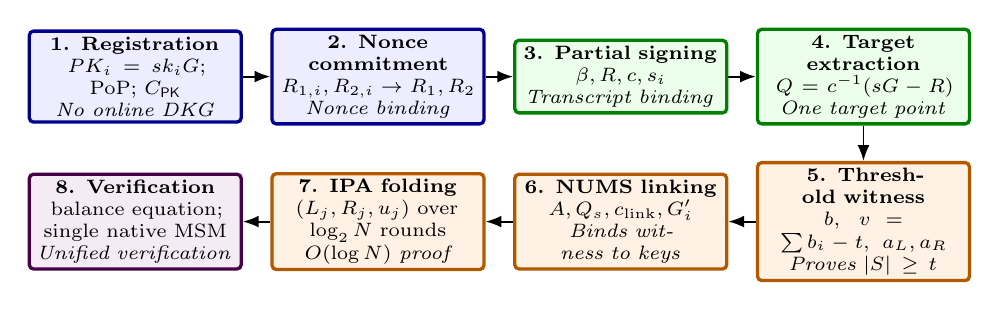
\begin{tikzpicture}[
  font=\scriptsize,
  cryptbox/.style={
    draw, rounded corners=1.5pt, very thick,
    align=center, text width=2.55cm, minimum height=0.82cm,
    inner sep=2pt
  },
  arr/.style={-{Latex[length=2mm]}, line width=0.7pt},
  setup/.style={cryptbox, fill=blue!7, draw=blue!55!black},
  sign/.style={cryptbox, fill=green!8, draw=green!50!black},
  proof/.style={cryptbox, fill=orange!10, draw=orange!70!black},
  verify/.style={cryptbox, fill=violet!8, draw=violet!55!black}
]
\node[setup] (r1) {\textbf{1. Registration}\\$PK_i=sk_iG$; PoP; $\CPK$\\{\scriptsize\itshape No online DKG}};
\node[setup, right=3.5mm of r1] (r2) {\textbf{2. Nonce commitment}\\$R_{1,i},R_{2,i}\rightarrow R_1,R_2$\\{\scriptsize\itshape Nonce binding}};
\node[sign, right=3.5mm of r2] (r3) {\textbf{3. Partial signing}\\$\beta,R,c,s_i$\\{\scriptsize\itshape Transcript binding}};
\node[sign, right=3.5mm of r3] (r4) {\textbf{4. Target extraction}\\$Q=c^{-1}(sG-R)$\\{\scriptsize\itshape One target point}};

\node[proof, below=4.5mm of r4] (r5) {\textbf{5. Threshold witness}\\$b,\;v=\sum b_i-t,\;a_L,a_R$\\{\scriptsize\itshape Proves $|S|\ge t$}};
\node[proof, left=3.5mm of r5] (r6) {\textbf{6. NUMS linking}\\$A,Q_s,c_{\rm link},G'_i$\\{\scriptsize\itshape Binds witness to keys}};
\node[proof, left=3.5mm of r6] (r7) {\textbf{7. IPA folding}\\$(L_j,R_j,u_j)$ over $\log_2N$ rounds\\{\scriptsize\itshape $O(\log N)$ proof}};
\node[verify, left=3.5mm of r7] (r8) {\textbf{8. Verification}\\balance equation; single native MSM\\{\scriptsize\itshape Unified verification}};

\draw[arr] (r1)--(r2);
\draw[arr] (r2)--(r3);
\draw[arr] (r3)--(r4);
\draw[arr] (r4)--(r5);
\draw[arr] (r5)--(r6);
\draw[arr] (r6)--(r7);
\draw[arr] (r7)--(r8);
\end{tikzpicture}
\end{center}

\captionof{figure}{Protocol at a glance: registration/setup (blue), Schnorr
signing (green), threshold proof generation (orange), and verification
(violet).}

\subsection{Logarithmic IPA folding and verification}

Over $\log_2N$ rounds, the prover recursively folds the witness and generator
vectors. Representative cross terms are
\[
L=\ip{a_{L,\mathrm{lo}}}{G'_{\mathrm{hi}}}+
\ip{a_{R,\mathrm{hi}}}{H_{\mathrm{lo}}}+\cdots,\qquad
R=\ip{a_{L,\mathrm{hi}}}{G'_{\mathrm{lo}}}+
\ip{a_{R,\mathrm{lo}}}{H_{\mathrm{hi}}}+\cdots .
\]
With transcript challenge $u$, folding uses
\[
a_L'=a_{L,\mathrm{lo}}u+a_{L,\mathrm{hi}}u^{-1}.
\]
The proof contains $2\log_2N$ curve points plus terminal scalars. Verification
reduces the resulting relation to a native MSM:
\[
\sum_{i=1}^{N}\lambda_iG_{\mathrm{nums},i}
+\sum_{i=1}^{n}(\lambda_i c_{\mathrm{link}})PK_i
+\sum_{j=1}^{M}\gamma_jK_j
\stackrel{?}{=}\Id.
\]

% \section{Implementation and Results}

% The above scheme is a \textbf{proposed construction}; no experimental benchmark is
% claimed yet. Its expected saving is in removing online DKG coordination,
% while the added zero-knowledge proof requires $O(\log N)$ IPA rounds.

% \textbf{Notation:} $n$ denotes the total number of participants, while $t$ denotes
% the minimum number of participants required to generate a valid threshold
% signature. $N$ denotes the dimension of the vector used in the IPA construction,
% and $M$ denotes the number of additional group-element terms contributing to
% the verification MSM. Here, MSM denotes multi-scalar multiplication.

% \begin{table}[!ht]
% \centering
% \scriptsize
% \renewcommand{\arraystretch}{1.08}
% \setlength{\tabcolsep}{3pt}
% \begin{tabular}{p{0.16\textwidth}p{0.19\textwidth}p{0.17\textwidth}p{0.19\textwidth}p{0.22\textwidth}}
% \toprule
% \textbf{Scheme} & \textbf{Setup} & \textbf{Signing} &
% \textbf{Verification} & \textbf{Time-saving opportunity}\\
% \midrule
% FROST & DKG / shares & $O(t)$ & $O(t)$ & No DKG saving\\
% MuSig2 & No DKG & $O(t)$ & $O(t)$ & Low setup cost; not $t$-of-$n$\\
% Threshold ECDSA & MPC setup & MPC-dependent & MPC-dependent & No direct setup saving\\
% Threshold BLS & Shared secret & $O(t)$ + pairing & Pairing-dependent & No direct setup saving\\
% \textbf{Proposed} & \textbf{No online DKG} & $\mathbf{O(t+\log N)}$ & $\mathbf{O(n+M+N)}$ MSM & \textbf{Removes online DKG; adds ZK/IPA work}\\
% \bottomrule
% \end{tabular}
% \caption{Expected asymptotic cost and time-saving opportunity; not measured benchmarks.}
% \label{tab:complexity}
% \end{table}% ============================================================
% 7. CONCLUSION
% ============================================================
\section{Conclusion}

The proposed DKG-free threshold Schnorr scheme combines independent keys,
silent setup, and a zero-knowledge threshold proof. It derives
$Q=c^{-1}(sG-R)=\sum_{i\in S}PK_i$ and proves $|S|\ge t$ without revealing the
signer set. The expected saving is removal of online DKG coordination, traded
for additional ZK/IPA computation; implementation and benchmarking are still
required.

\begin{thebibliography}{99}

\bibitem{Schnorr}
C.-P. Schnorr, ``Efficient Signature Generation by Smart Cards,''
\emph{Journal of Cryptology}, vol. 4, no. 3, pp. 161--174, 1991.

\bibitem{Wagner}
D. A. Wagner, ``A Generalized Birthday Problem,''
in \emph{CRYPTO 2002}, LNCS, pp. 288--303, Springer, 2002.

\bibitem{MuSig2}
J. Nick, T. Ruffing, and Y. Seurin,
``MuSig2: Simple Two-Round Schnorr Multi-signatures,''
in \emph{CRYPTO 2021}, LNCS 12825, pp. 189--221, 2021.

\bibitem{FROST}
C.-P. Connolly et al.,
``The Flexible Round-Optimized Schnorr Threshold (FROST) Protocol,''
IETF RFC 9591, 2024.

\bibitem{Bulletproofs}
B. B{\"u}nz et al.,
``Bulletproofs: Short Proofs for Confidential Transactions and More,''
in \emph{IEEE Symposium on Security and Privacy}, pp. 315--334, 2018.

\bibitem{KZG}
A. Kate, G. M. Zaverucha, and I. Goldberg,
``Constant-Size Commitments to Polynomials and Their Applications,''
in \emph{ASIACRYPT 2010}, pp. 177--194, 2010.

\bibitem{hinTS}
S. Garg et al.,
``hinTS: Threshold Signatures with Silent Setup,''
in \emph{IEEE Symposium on Security and Privacy},
pp. 3034--3052, 2024.

\bibitem{GennaroGoldfeder}
R. Gennaro and S. Goldfeder,
``Fast Multiparty Threshold ECDSA with Fast Trustless Setup,''
in \emph{ACM CCS}, 2018.

\bibitem{ThBLS}
M. Hajiabadi et al.,
``On the Adaptive Security of the Threshold BLS Signature Scheme,''
Cryptology ePrint Archive, Report 2022/534, 2022.

\end{thebibliography}

\end{document}